%%%%%%%%%%%%%%%%%%%%%%%%%%%%%%%%%%%%%%%%%%%%%%%%%%%%%%%%%%%%%%%%%%%%%%
% How to use writeLaTeX: 
%
% You edit the source code here on the left, and the preview on the
% right shows you the result within a few seconds.
%
% Bookmark this page and share the URL with your co-authors. They can
% edit at the same time!
%
% You can upload figures, bibliographies, custom classes and
% styles using the files menu.
%
%%%%%%%%%%%%%%%%%%%%%%%%%%%%%%%%%%%%%%%%%%%%%%%%%%%%%%%%%%%%%%%%%%%%%%

\documentclass[12pt]{article}

\usepackage{sbc-template}
\usepackage{graphicx,url}
\usepackage{listings}
\usepackage{xcolor}

% Definindo novas cores
\definecolor{verde}{rgb}{0,0.5,0}

% Configurando layout para mostrar códigos C
\lstdefinelanguage{C}{%
  morekeywords={break,case,catch,char,const,continue,default,do,double,else,enum,extern,float,for,friend,goto,if,inline,int,long,namespace,new,operator,override,private,protected,public,register,return,short,signed,sizeof,static,struct,switch,template,this,throw,true,false,try,typedef,union,unsigned,using,virtual,void,volatile,wchar_t,while},%
  sensitive=true,%
  morestring=[b]",%
  morecomment=[l]//,%
  morecomment=[s]{/*}{*/},%
}

\lstset{
  language=C, %indicar a linguagem utilizada
  basicstyle=\ttfamily\tiny, 
  keywordstyle=\color{blue}, 
  stringstyle=\color{verde}, 
  commentstyle=\color{gray}, 
  extendedchars=true, 
  showspaces=false, 
  showstringspaces=false, 
  numbers=left,
  numberstyle=\tiny,
  breaklines=true, 
  breakautoindent=true, 
  captionpos=b,
  xleftmargin=0pt,
  frame=single,
}

% Mudando o nome da listagem em codigo; pode-se mudar para outro nome tambem
\renewcommand{\lstlistingname}{Listagem}
\renewcommand{\figurename}{Figura}
\renewcommand{\tablename}{Tabela}

%\usepackage[brazil]{babel}   
\usepackage[utf8]{inputenc}  

     
\sloppy

\title{Demonstração e Apresentação de Desempenho de Modelos de Difusão de Contaminantes em Água}

\author{Fernando Daniel Marcelino\inst{1}, Lucas Moura da Silva\inst{1},\\ Marcos Vinicius Gasparoto Bauab\inst{1} }


\address{Universidade Federal de São Paulo -- Campus São José dos Campos\\
Avenida Cesare Mansueto Giulio Lattes, 1201 -Eugênio de Mello\\
São José dos Campos/SP - CEP: 12247-014
  \email{\{fernando.marcelino,lucas.silva16,marcos.bauab\}@unifesp.br}
}

\begin{document} 

\maketitle

%\begin{abstract}
%The contamination of water resources by pollutants represents one of the most critical environmental issues today, significantly affecting public health and global biodiversity, with particularly severe impacts in developing countries. The diffusion of contaminants in water bodies is a complex phenomenon that can be modeled using partial differential equations. This study presents an approximate model for contaminant diffusion in water, implemented in the C programming language and parallelized using NVIDIA's CUDA. Performance tests were conducted to evaluate the impact of parallelization on the model's execution time, and the results demonstrated that parallelization was highly effective in reducing execution time. Thus, the study highlights the relevance of GPU-based parallel architectures for solving environmental problems that require high computational power.
%\end{abstract}
     
\begin{resumo} 
A contaminação dos recursos hídricos por poluentes representa um dos mais graves problemas ambientais da atualidade, afetando significativamente a saúde pública e a biodiversidade global, com impacto especialmente severo em países em desenvolvimento. A difusão de contaminantes em corpos d'água é um fenômeno complexo que pode ser modelado por equações diferenciais parciais. Neste trabalho, é apresentado um modelo aproximado de difusão de contaminantes em água, implementado na linguagem C e paralelizado utilizando OpenMP, CUDA e MPI. Foram realizados testes de desempenho para avaliar o impacto da paralelização no tempo de execução do modelo, e os resultados obtidos mostraram que a paralelização foi eficaz na redução do tempo de execução, para algumas metodologias. Assim, destaca-se a relevância do uso de arquiteturas paralelas baseadas em GPUs para a solução de problemas ambientais que demandam alto poder computacional.
\end{resumo}

% Seção de Introdução
\section{Introdução} \label{sec:introducao}

A contaminação da água é um problema ambiental crítico que afeta a saúde pública, a biodiversidade e a economia global. Trata-se de uma questão que preocupa grandes órgãos nacionais e internacionais, como a Organização das Nações Unidas (ONU). Em 2015, os países-membros da ONU comprometeram-se com um apelo universal à ação para erradicar a pobreza, proteger o planeta e garantir que, até 2030, todas as pessoas desfrutem de paz e prosperidade. Contudo, em virtude do aumento das atividades industriais, agrícolas e urbanas, a quantidade de poluentes lançados nos corpos d’água tem crescido significativamente, tornando essencial o desenvolvimento de modelos eficazes para prever a difusão de contaminantes.

Diante desse cenário, modelos computacionais de difusão de contaminantes em água são ferramentas fundamentais para entender e prever o comportamento de poluentes. Esses modelos permitem simular a dispersão de substâncias químicas, biológicas e físicas em rios, lagos, aquíferos e oceanos, fornecendo informações valiosas para a gestão ambiental e a tomada de decisões. No entanto, tais simulações frequentemente demandam alto custo computacional, especialmente quando realizadas em grande escala ou com alta precisão.

Para enfrentar esse desafio computacional, este trabalho explora três abordagens de computação paralela: a \emph{API OpenMP (Open Multi-Processing)} para processamento em CPU \emph{multicore}, a arquitetura \emph{CUDA (Compute Unified Device Architecture)} da NVIDIA para processamento em GPUs, e o padrão \emph{MPI (Message Passing Interface)} para sistemas distribuídos. A escolha dessas tecnologias justifica-se pela sua complementaridade: enquanto o \emph{OpenMP} simplifica a paralelização em sistemas com memória compartilhada, o \emph{CUDA} explora o paralelismo massivo de GPUs para cálculos matriciais intensivos, e o \emph{MPI} permite escalabilidade em clusters heterogêneos, onde processos independentes comunicam-se por troca de mensagens \cite{gropp:2014, mpi:2020}.

O objetivo deste trabalho é apresentar uma análise detalhada e comparativa entre quatro implementações do modelo de difusão de contaminantes: uma versão sequencial (\emph{baseline}), uma versão paralela utilizando \emph{OpenMP}, outra com \emph{CUDA} e uma quarta com \emph{MPI}. O modelo adapta-se às condições dos fluidos e de variáveis físicas, como volume amostral e coeficiente de difusão. A implementação base foi realizada em C/C++, e foram conduzidos testes extensivos de desempenho em diferentes configurações de \emph{hardware}, incluindo ambientes distribuídos para avaliação do \emph{MPI}. Os resultados são analisados em termos de tempo de execução, \emph{speedup}, eficiência de paralelização e escalabilidade, destacando cenários onde cada tecnologia se mostra mais adequada.

% Seção de Fundamentação Teórica
\section{Fundamentação Teórica} \label{sec:fundaTeorica}
A fundamentação teórica deste trabalho aborda os conceitos essenciais e as ferramentas utilizadas na implementação do modelo matemático de difusão de contaminantes, com ênfase nas técnicas de programação paralela. Até o presente momento, os modelos propostos foram desenvolvidos utilizando o OpenMP, CUDA e MPI. Ambas as aplicações, diferem em suas abordagens de paralelização, mas compartilham o objetivo de otimizar o tempo de execução do modelo. A seguir, são apresentados os conceitos fundamentais de cada tecnologia, bem como suas características e aplicações.

\subsection{OpenMP} \label{subsec:openmp}
A programação concorrente e distribuída pode ser feita de várias formas, e a principal maneira de se implementar é utilizando de \emph{threads}. Para isso, também existem tecnologias consolidadas na academia e na indústria de software para aplicações de alto desempenho, como as \emph{Application Programming Interface} (API) para programação paralela. Uma dessas tecnologias é o \emph{OpenMP} (\emph{Open Multi-Processing}), que é uma API de programação paralela de memória compartilhada, que permite a paralelização de laços de repetição, blocos de código e funções e outros \cite{chapman:2007}.

O \emph{OpenMP} pode ser utilizada para as linguagens de programação Fortran, C/C++, possuindo formatos específicos em suas diretivas e funcionalidades. Sua programação é organizada igual à programas sequenciais, tornando a sintaxe muito fácil de ser entendido por usuários conencionais de aplicações lineares \cite{gropp:2017}.

Para se utizar dos benefícios da programação pela \emph{API} \emph{OpenMP}, é necessário a utilização de diretivas, que são instruções que são interpretadas pelo compilador, e que são utilizadas para a paralelização de trechos de código. As diretivas em C/C++ são precedidas por:

\begin{minipage}[t]{0.48\textwidth}
  \begin{verbatim}
    // Em C/C++
    #pragma omp
  \end{verbatim}
  \end{minipage}
\hfill
\begin{minipage}[t]{0.48\textwidth}
  \begin{verbatim}
    // Em Fortran
    !$omp
  \end{verbatim}
  \end{minipage}

Após a declaração do formato descrito, é preciso utilizar de parâmetros e diretivas para que se consigo utilizar a tecnologia. Algumas diretivas amplamente utilizadas são:

\begin{minipage}[t]{0.48\textwidth}
  \begin{verbatim}
    parallel
    for
    critical
    atomic
    private
  \end{verbatim}
  \end{minipage}
\hfill
\begin{minipage}[t]{0.48\textwidth}
  \begin{verbatim}
    shared
    reduction
    schedule
    barrier
    num_threads
  \end{verbatim}
  \end{minipage}

A listagem completa das diretivas e métodos acessadas pela \emph{API} pode ser encontra nos guias de referências\footnote{O guia de referência da \emph{Open MP API} é um documento que abrange todas as possíveis implementações realizadas pela tecnologia. Pode ser encontradas na \emph{web} pelo endereço www.openmp.org/resources/refguides/} da \emph{OpenMP}.

\subsubsection{Diretivas}
As principais diretivas do OpenMP incluem:

\begin{itemize}
    \item \texttt{parallel}: Cria uma região paralela onde múltiplas threads executam simultaneamente.
    \item \texttt{for}: Distribui as iterações de um loop entre threads disponíveis.
    \item \texttt{collapse(n)}: Combina múltiplos loops aninhados em uma única iteração paralela.
    \item \texttt{reduction}: Executa operações de redução (como soma, produto) de forma segura entre threads.
    \item \texttt{schedule}: Define como as iterações são distribuídas entre as threads:
        \begin{itemize}
            \item \texttt{static}: Divide as iterações igualmente entre threads.
            \item \texttt{dynamic}: Distribui iterações sob demanda.
            \item \texttt{guided}: Usa blocos de tamanho decrescente.
        \end{itemize}
    \item \texttt{private}: Cria cópias locais de variáveis para cada thread.
    \item \texttt{shared}: Permite que todas as threads acessem a mesma variável.
    \item \texttt{critical}: Define uma região que só pode ser executada por uma thread por vez.
    \item \texttt{barrier}: Sincroniza todas as threads em um ponto específico.
\end{itemize}

Estas diretivas são fundamentais para controlar a execução paralela e garantir o correto compartilhamento de dados entre threads.


\subsection{CUDA}
A computação convencional baseada em CPUs utiliza um modelo de processamento sequencial, no qual as instruções são executadas em uma ordem predefinida. Contudo, essa abordagem começou a ser complementada à medida que a demanda por processamento de dados e instruções aumentou, exigindo uma quebra de paradigma na programação. Ao longo dos anos, esse novo paradigma foi amplamente adotado em áreas como processamento de imagens, simulações físicas, aprendizado de máquina e outras aplicações que requerem elevado poder de processamento. Dessa forma, iniciaram-se os estudos e o desenvolvimento de tecnologias de processamento gráfico, conhecidas como \emph{Graphics Processing Units} (GPUs).

Na década de 1970, começaram os primeiros desenvolvimentos voltados ao processamento gráfico, e, um pouco antes dos anos 2000, consolidaram-se estudos que deram origem à arquitetura das GPUs modernas. Com isso, arquiteturas heterogêneas GPU-CPU passaram a ser empregadas em aplicações de alto desempenho \cite{cheng:2014}. 

Com o avanço das GPUs, identificou-se que elas poderiam ser utilizadas para programação de propósito geral, e não apenas para processamento gráfico. A NVIDIA foi uma das pioneiras no desenvolvimento de tecnologias para essa finalidade, introduzindo a \emph{Compute Unified Device Architecture} (CUDA). Desenvolvida em 2006, a CUDA é uma plataforma de computação paralela que permite a programação de GPUs NVIDIA para aplicações de alto desempenho \cite{cuda:2012}. A programação em CUDA é realizada em C/C++, e a plataforma oferece um conjunto de ferramentas, manuais e bibliotecas que facilitam o desenvolvimento de aplicações paralelas.

\subsubsection{Núcleos de Processamento} \label{subsubsec:cuda_cores}
O processamento em CUDA é realizado por meio da execução de um \emph{kernel}, que é uma função especial criada na CPU e executada na GPU. O \emph{kernel} é executado por um grande número de \emph{threads} em paralelo, sendo que cada \emph{thread} é processada por um núcleo da GPU. Os núcleos de processamento são organizados em blocos, enquanto os blocos são dispostos em \emph{grids}. A invocação de um \emph{kernel} em CUDA utiliza uma notação especial, com os parâmetros envolvidos entre os delimitadores \texttt{<<<} e \texttt{>>>}, onde o primeiro parâmetro especifica o número de blocos e o segundo, o número de \emph{threads} por bloco.

\vspace{0.5cm}
\begin{lstlisting}[language=C, caption={Exemplo de definição e invocação de um kernel CUDA para adição vetorial}, label={lst:cuda_kernel_example}]
__global__ void VecAdd(float* A, float* B, float* C)
{
  int i = threadIdx.x;
  C[i] = A[i] + B[i];
}

int main()
{
  ...
  // Kernel invocation with N threads
  VecAdd<<<1, N>>>(A, B, C);
  ...
}
\end{lstlisting}
\vspace{0.5cm}

O código apresentado na Listagem~\ref{lst:cuda_kernel_example} ilustra um exemplo de definição e invocação de um \emph{kernel} CUDA para adição vetorial. Nesse exemplo, utiliza-se apenas um bloco contendo \emph{N threads}. O \emph{kernel} recebe três vetores de ponto flutuante como parâmetros (\emph{A}, \emph{B} e \emph{C}) e realiza a soma elemento a elemento dos vetores \emph{A} e \emph{B}, armazenando o resultado no vetor \emph{C}. O índice para percorrer os elementos dos vetores é unidimensional; entretanto, em problemas clássicos como a multiplicação de matrizes, os índices podem ser bidimensionais ou até tridimensionais. 

A organização hierárquica dos blocos e \emph{threads} exige o cálculo dos índices para acessar corretamente os elementos das estruturas de dados. O acesso às \emph{threads} é feito utilizando as funções \emph{threadIdx.x}, \emph{threadIdx.y} e \emph{threadIdx.z}, em conjunto com \emph{blockIdx.x}, \emph{blockIdx.y} e \emph{blockIdx.z}, bem como \emph{blockDim.x}, \emph{blockDim.y} e \emph{blockDim.z}. Essa combinação permite o mapeamento completo das \emph{threads} processadas pela GPU.

Um exemplo esquemático da organização de blocos e \emph{threads} em CUDA é apresentado na Figura~\ref{fig:gridblock_thread}. A figura ilustra a identificação de \emph{threads} e blocos em uma grade de 2x2 blocos, onde cada bloco contém 4x4 \emph{threads}.

\begin{figure}[ht]
  \centering
  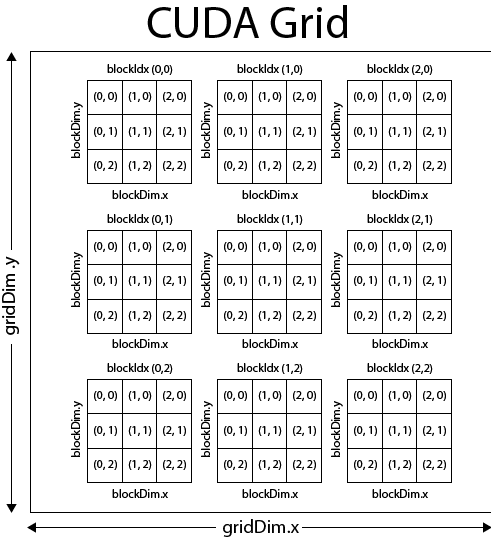
\includegraphics[width=0.65\textwidth]{imagens/gridblock_thread.png}
  \caption{Esquema de identificação de \emph{threads} e blocos em CUDA. \cite{mckennon:2013}}
  \label{fig:gridblock_thread}
\end{figure}

\subsubsection{GPU} \label{subsec:gpu}
A Unidade de Processamento Gráfico (\emph{Graphics Processing Unit}, GPU) é um processador especializado no aceleramento de processamento gráfico, especialmente em aplicações como renderização 3D e processamento de imagens. Com o avanço das arquiteturas computacionais, as GPUs evoluíram para plataformas de computação paralela de propósito geral, amplamente utilizadas em ciência de dados, aprendizado de máquina, simulações físicas e outras aplicações de alta performance, conhecidas como \emph{General-Purpose Graphics Processing Unit} (GPGPU). \cite{owens:2008}

Enquanto as CPUs são otimizadas para latência, as GPUs são projetadas para lidar com várias \emph{threads} simultaneamente, devido à sua arquitetura massivamente paralela. Isso ocorre porque a GPU é composta por centenas ou milhares de núcleos organizados em múltiplos blocos, chamados de \emph{Streaming Multiprocessors} (SMs). Cada SM é projetado para executar centenas de \emph{threads} em paralelo, adotando um modelo de execução baseado em \emph{Single Instruction, Multiple Thread} (SIMT), que é uma das classificações da taxonomia de Flynn.

\subsubsection{GPU T4} \label{subsubsec:gpu_t4}
As GPUs T4, baseadas na arquitetura Turing da NVIDIA, representam um avanço significativo no uso de GPUs para computação de propósito geral e aprendizado de máquina. A T4 foi projetada como uma solução otimizada para data centers modernos, suportando cargas de trabalho mistas que incluem treinamento, inferência, virtualização e serviços baseados em inteligência artificial (IA).

A GPU T4 possui 49 KB de memória compartilhada, 4 MB de memória cache L2 e um tamanho de \emph{warp} de 32 \emph{threads}, ou seja, a quantidade de \emph{threads} que podem ser usadas simultaneamente. O número máximo de \emph{threads} por bloco e por multiprocessador é de 1024, e a GPU conta com 40 multiprocessadores. A dimensão máxima de \emph{threads} por bloco é (1024, 1024, 64) nos eixos (x, y, z), enquanto o \emph{grid} possui dimensão máxima de (2147483647, 65535, 65535).

A Figura~\ref{fig:archT4} apresenta o esquemático da configuração da arquitetura da NVIDIA Tesla T4.

\begin{figure}[ht]
  \centering
  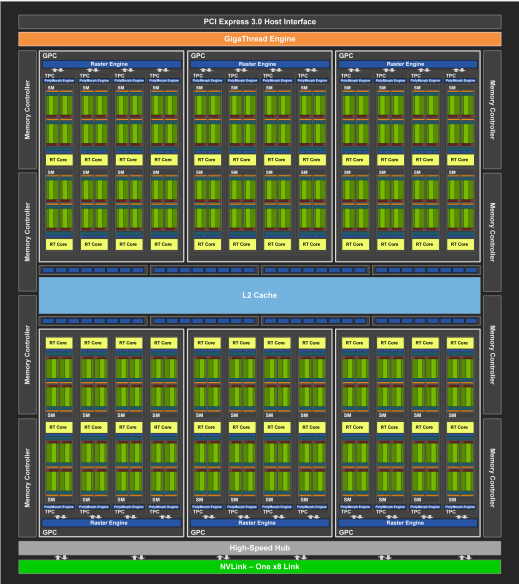
\includegraphics[width=0.6\textwidth]{imagens/gpu-t4.png}
  \caption{Arquitetura da GPU Tesla T4. \cite{nvidia:2018}}
  \label{fig:archT4}
\end{figure}


\subsection{Message Passing Interface (MPI)} \label{subsec:mpi}
Diferentemente do paradigma pro programação realizado em CUDA, o MPI é uma biblioteca de comunicação de mensagens que permite a execução de programas paralelos em sistemas distribuídos. A biblioteca possui semânticas para interfaces de programação em C e Fortran, com uma ampla gama de funções no padrão MPI. Com isso, processos podem estar sendo executados em sistemas operacionais diferentes, em diferentes arquiteturas de hardware e até mesmo em diferentes locais geográficos, diferentemente das outras abordagens encontradas para se fazer concorrência.  O MPI é amplamente utilizado em supercomputadores e clusters de computadores, permitindo a comunicação entre processos independentes que executam em diferentes nós de um sistema distribuído. \cite{gropp:2014}

Analogamente ao CUDA, o MPI também possui uma estrutura hierárquica, onde os processos são organizados em grupos chamados \emph{communicators}. Cada \emph{communicator} possui um identificador único, que é utilizado para a comunicação entre os processos. A comunicação entre processos é realizada por meio de funções de envio e recebimento de mensagens, como \texttt{MPI\_Send} e \texttt{MPI\_Recv}, que permitem a troca de dados entre processos de forma síncrona ou assíncrona. Portanto, antes mesmo de fazer a transmissão em paralela dos processos, deve-se utilizar ferramentas de sincronização para garantir que a comunicação entre os processos seja feita de forma correta. A Listagem \ref{lst:mpi_example} apresenta um exemplo de código que utiliza a biblioteca MPI para realizar a inicialização, sincronizações e finalização dos processos.

\vspace{0.5cm}
\begin{lstlisting}[language=C, caption={Exemplo de código MPI.}, label={lst:mpi_example}]
#include <mpi.h>
#include <stdio.h>

int main(int argc, char** argv) {
    int rank, size;

    // Iniciando o ambiente MPI e obtendo o rank e o tamanho do comunicador conforme as entradas
    MPI_Init(&argc, &argv);

    MPI_Comm_rank(MPI_COMM_WORLD, &rank);
    MPI_Comm_size(MPI_COMM_WORLD, &size);

    // Procedimento a ser realizado por cada processo
    printf("Hello, world! I am %d of %d\n", rank, size);

    // Finalizando o ambiente MPI
    MPI_Finalize();

    return 0;
}
\end{lstlisting}
\vspace{0.5cm}

\subsubsection{Funcionalidades MPI} \label{subsubsec:mpi_funcionalidades}
Os tipos de dados e funções disponíveis na biblioteca MPI permitem a comunicação entre processos de forma eficiente e segura, mas é necessário um conhecimento prévio sobre a biblioteca para utilizá-la corretamente. Com isso, será apresentado brevemente as principais funções e tipos de dados utilizados na biblioteca MPI.

As principais funções do MPI incluem:
\begin{itemize}
    \item \texttt{MPI\_Init}: Inicializa o ambiente MPI. Recebe argumentos da linha de comando e deve ser chamada antes de qualquer outra função MPI.
    \item \texttt{MPI\_Finalize}: Finaliza o ambiente MPI. É a última função MPI a ser chamada, limpando recursos alocados.
    \item \texttt{MPI\_Comm\_size}: Retorna o número total de processos em um comunicador específico.
    \item \texttt{MPI\_Comm\_rank}: Retorna o identificador único (rank) do processo atual dentro do comunicador.
    \item \texttt{MPI\_Send}: Envia uma mensagem para outro processo, especificando buffer, tipo de dado, destino e tag.
    \item \texttt{MPI\_Recv}: Recebe uma mensagem de outro processo, armazenando os dados em um buffer.
    \item \texttt{MPI\_Barrier}: Bloqueia a execução até que todos os processos no comunicador atinjam este ponto, garantindo sincronização.
\end{itemize}

\begin{table}[ht]
    \centering
    \caption{Principais Tipos de Dados MPI}
    \begin{tabular}{|c|c|}
        \hline
        \textbf{Tipo de Dado} & \textbf{Descrição} \\
        \hline
        \texttt{MPI\_CHAR} & Representa um caractere \\
        \hline
        \texttt{MPI\_INT} & Representa um inteiro \\
        \hline
        \texttt{MPI\_FLOAT} & Representa um número de ponto flutuante de precisão simples \\
        \hline
        \texttt{MPI\_DOUBLE} & Representa um número de ponto flutuante de precisão dupla \\
        \hline
        \texttt{MPI\_LONG} & Representa um número inteiro longo \\
        \hline
        \texttt{MPI\_UNSIGNED} & Representa um número inteiro sem sinal \\
        \hline
        \texttt{MPI\_BYTE} & Representa um byte \\
        \hline
        \texttt{MPI\_PACKED} & Representa dados empacotados \\
        \hline
    \end{tabular}
    \label{tab:mpi_data_types}
\end{table}

Além desses tipos de dados básicos, a biblioteca MPI permite a definição de tipos de dados derivados, que são combinações de tipos de dados básicos. Isso é útil para enviar e receber estruturas de dados complexas. As funções \texttt{MPI\_Type\_contiguous}, \texttt{MPI\_Type\_vector}, \texttt{MPI\_Type\_indexed}, entre outras, são utilizadas para criar esses tipos de dados derivados.


\subsection{Stencil} \label{subsec:stencil}
O stencil é uma abordagem de programação paralela que consiste em aplicar uma operação a cada elemento de um conjunto de dados, utilizando os valores dos elementos vizinhos, conforme um raio de vizinhança predefinido. Essa técnica é particularmente útil em simulações numéricas que envolvem equações diferenciais parciais, como no caso da difusão de contaminantes em água. A computação baseada em stencil é altamente paralelizável, pois cada elemento pode ser processado independentemente, desde que os valores dos vizinhos estejam disponíveis. \cite{cruz:2015}

A abordagem do \emph{stencil} é amplamente utilizado em diversas áreas da ciência computacional, como geofísica, astrofísica, física nuclear e oceanografia. Essas áreas demandam simulações computacionais em larga escala, com alta frequência de saída. Quando equações diferenciais parciais (EDPs) são empregadas, elas geralmente são resolvidas pelo método das diferenças finitas, utilizando o \emph{stencil} para calcular os operadores diferenciais, que representam uma parcela significativa do tempo total de execução.

No uso do \emph{stencil}, para cada ponto de um conjunto de dados, como em uma matriz bidimensional (2D), são considerados os pesos dos pontos vizinhos para resolver os operadores diferenciais espacialmente, como ilustrado na Figura~\ref{fig:stencil_2d}. Dessa forma, replicando essas operações para todos os pontos do conjunto, é possível realizar a paralelização ideal, onde cada \emph{thread} calcula o valor correspondente a um ponto. Isso possibilita a paralelização eficiente do código, reduzindo significativamente o tempo de execução. \cite{cruz:2015}

\begin{figure}[ht]
  \centering
  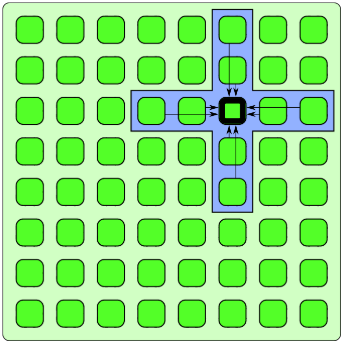
\includegraphics[width=0.5\textwidth]{imagens/stencil_2d-teoric.png}
  \caption{Exemplo de stencil 2D. \cite{phdthesis:2018}}
  \label{fig:stencil_2d}
\end{figure}



% Seção de Desenvolvimento
\section{Desenvolvimento} \label{sec:desenvolvimento}

A simulação de um modelo de difusão de contaminantes em água pode ser equacionado por:

\[
\frac{\partial C}{\partial t} + \mathbf{v} \cdot \nabla C = D \nabla^2 C
\]

Onde:
\begin{itemize}
    \item \( C \) é a concentração do contaminante.
    \item \( t \) é o tempo (em segundos).
    \item \( \mathbf{v} \) é o vetor de velocidade do fluxo da água.
    \item \( D \) é o coeficiente de difusão do contaminante na água.
    \item \( \nabla^2 C \) é a ataxa de variação da concentração no espaço.
\end{itemize}

Ou ainda, pode ser formulada de uma modo mais extenso

\[
C^{(t+1)}_{i,j} = C^{(t)}_{i,j} + D \cdot \Delta t \cdot \frac{C^{(t)}_{i+1,j} + C^{(t)}_{i-1,j} + C^{(t)}_{i,j+1} + C^{(t)}_{i,j-1} - 4 \cdot C^{(t)}_{i,j}}{\Delta x^2}
\]

A parte mais importante do código pode ser observada na Listagem~\ref{lst:diffusion}, onde é resaltado os calculos para a concentração da iteração \emph{i+1}.

\begin{lstlisting}[language=C, caption={Código da Equação de Difusão em C}, label=lst:diffusion]
void diff_eq(double **C, double **C_new) {
    for (int t = 0; t < T; t++) {
        for (int i = 1; i < N - 1; i++) {
            for (int j = 1; j < N - 1; j++) {
                C_new[i][j] = C[i][j] + D * DELTA_T * (
                    (C[i+1][j] + C[i-1][j] + C[i][j+1] + C[i][j-1] - 4 * C[i][j]) / (DELTA_X * DELTA_X)
                );
            }
        }
        // Atualizar matriz para a proxima iteracao
        double difmedio = 0.;
        for (int i = 1; i < N - 1; i++) {
            for (int j = 1; j < N - 1; j++) {
                difmedio += fabs(C_new[i][j] - C[i][j]);
                C[i][j] = C_new[i][j];
            }
        }
        if ((t%100) == 0)
          printf("interacao %d - diferenca=%g\n", t, difmedio/((N-2)*(N-2)));
    }
}
\end{lstlisting}

Para alocar o máximo de espaço para a matriz bidimensional, foi necessário alocar memória de forma dinâmica para evitar que ocorra \emph{segmentation fault (core dumped)} com valores altos, como mostra a Listagem~\ref{lst:matrix_allocation_memory}. Isso também se aplica à matriz da próxima iteração, ou seja, \emph{C\_new}. Ambas as matrizes começam com 0 em todas as posições, e para a matriz \emph{C}, há uma grande concentração no seu centro, igual a 1,0.

\begin{lstlisting}[language=C, caption={Alocação de memória para a matriz}, label={lst:matrix_allocation_memory}]
// Concentracao inicial
double **C = (double **)malloc(N * sizeof(double *));
if (C == NULL) {
    fprintf(stderr, "Memory allocation failed\n");
    return 1;
}
for (int i = 0; i < N; i++) {
    C[i] = (double *)malloc(N * sizeof(double));
    if (C[i] == NULL) {
        fprintf(stderr, "Memory allocation failed\n");
        return 1;
    }
}
\end{lstlisting}

\subsection{Paralelizando com o OpenMP}
Para otimizar o código apresentado na Listagem~\ref{lst:diffusion_openmp}, foi utilizado o conceito de \emph{threads}, dividindo o cálculo da concentração de toda a matriz em \emph{n} \emph{threads}. A abordagem escolhida foi a utilização do \emph{OpenMP}, conforme mostrado na Listagem~\ref{lst:diffusion_openmp}. No primeiro conjunto de \emph{for}, em \emph{\#pragma omp parallel for}, são usadas duas cláusulas: \emph{collapse(2)}, que agrupa conjuntos de \emph{loops} sequenciais (neste caso, dois), e \emph{schedule(static)}, que divide as iterações do \emph{for} de forma igual entre as \emph{threads}.

Já no segundo conjunto de \emph{for}, há mais uma cláusula: \emph{reduction(+:difmedio)}, que faz a redução do \emph{difmedio}. Assim, cada \emph{thread} soma seu valor, e, no final, é necessário obter o valor resultante.

\begin{lstlisting}[language=C, caption={Código da Equação de Difusão em C com OpenMP}, label=lst:diffusion_openmp]
void diff_eq(double **C, double **C_new, int n_threads) {
    omp_set_num_threads(n_threads);
    for (int t = 0; t < T; t++) {
        #pragma omp parallel for collapse(2) schedule(static)
        for (int i = 1; i < N - 1; i++) {
            for (int j = 1; j < N - 1; j++) {
                C_new[i][j] = C[i][j] + D * DELTA_T * (
                    (C[i+1][j] + C[i-1][j] + C[i][j+1] + C[i][j-1] - 4 * C[i][j]) / (DELTA_X * DELTA_X)
                );
            }
        }

        double difmedio = 0.;
        #pragma omp parallel for collapse(2) reduction(+:difmedio) schedule(static)            
        for (int i = 1; i < N - 1; i++) {
            for (int j = 1; j < N - 1; j++) {
                difmedio += fabs(C_new[i][j] - C[i][j]);
                C[i][j] = C_new[i][j];
            }
        }
        if ((t%100) == 0)
            printf("interacao %d - diferenca=%g\n", t, difmedio/((N-2)*(N-2)));
    }
}
\end{lstlisting}

A configuração do número de \emph{threads}, é passada por parâmetro no executável do programa.

Outra abordagem utilizada para otimizar o tempo de execução do processo foi a mudança na alocação de memória dinâmica, como mostrado na Listagem~\ref{lst:matrix_allocation_memory_optimization}. Como pode ser visto na Figura~\ref{lst:matrix_allocation_memory}, é realizada uma alocação para um \emph{array} de \emph{double} de \emph{N} posições. Em seguida, é feita a alocação de outro \emph{array} de \emph{N} posições para cada posição do primeiro \emph{array}. Para melhorar isso, foi alocado apenas um único \emph{array} de \emph{N*N} posições, configurando a matriz desejada.

\begin{lstlisting}[language=C, caption={Alocação de memória para as matrizes de forma otimizada}, label={lst:matrix_allocation_memory_optimization}]
// Alocacao dinamica para as matrizes
double *C = (double *)malloc(N * N * sizeof(double));
double *C_new = (double *)malloc(N * N * sizeof(double));
\end{lstlisting}

Dessa forma, os cálculos para as concentrações também mudaram, mas apenas para atender às novas matrizes, como mostrado na Listagem~\ref{lst:diff_eq_openmp}.

\begin{lstlisting}[language=C, caption={Código otimizado da equação de difusão com OpenMP}, label=lst:diff_eq_openmp]
void diff_eq(double *C, double *C_new, int n_threads) {
    omp_set_num_threads(n_threads);
    double delta_x_squared_inv = 1.0 / (DELTA_X * DELTA_X);

    for (int t = 0; t < T; t++) {
        #pragma omp parallel for schedule(static)
        for (int i = 1; i < N - 1; i++) {
            for (int j = 1; j < N - 1; j++) {
                C_new[i * N + j] = C[i * N + j] + D * DELTA_T * (
                                    (C[(i+1) * N + j] + C[(i-1) * N + j] + C[i * N + (j+1)] + C[i * N + (j-1)] - 4 * C[i * N + j]) * 
                                    delta_x_squared_inv
                );
            }
        }

        double difmedio = 0.0;
        #pragma omp parallel for reduction(+:difmedio) schedule(static)
        for (int i = 1; i < N - 1; i++) {
            for (int j = 1; j < N - 1; j++) {
                difmedio += fabs(C_new[i * N + j] - C[i * N + j]);
                C[i * N + j] = C_new[i * N + j];
            }
        }

        if ((t%100) == 0)
            printf("interacao %d - diferenca=%g\n", t, difmedio/((N-2)*(N-2)));
    }
}
\end{lstlisting}



\subsection{Paralelizando com o CUDA}
No vigente trabalho, foram realizados duas abordagens em CUDA. A primeira foi a paralelização do \emph{stencil} 1D, e a segunda, do \emph{stencil} 2D. Ambas as abordagens utilizam a mesma equação de difusão, mas com diferentes implementações para a matriz de concentração.

\subsubsection{Stencil 1D}
\label{desenv:stencil1d}
O stencil 1D utiliza um vetor unidimensional para realizar os cálculos, garantindo que não sejam acessados espaços de memória inválidos.

\vspace{0.5cm}
\begin{lstlisting}[language=C, caption={Chamada do \emph{kernel}.}, label={lst:diff_eq}]
double diff_eq(double *C, double *C_new) {
    double *d_C, *d_C_new;
    double *swap, difmedio;

    cudaMalloc( (void **) &d_C, SIZE);
    cudaMalloc( (void **) &d_C_new, SIZE);

    cudaMemcpy(d_C, C, SIZE, cudaMemcpyHostToDevice );
    cudaMemcpy(d_C_new, C_new, SIZE, cudaMemcpyHostToDevice );

    for (int t = 0; t < T; t++) {
        diff_eq_kernel<<< (N * N + (THREADS_PER_BLOCK-1)) / THREADS_PER_BLOCK, THREADS_PER_BLOCK >>>(d_C, d_C_new, N);

        cudaDeviceSynchronize();

        swap = d_C;
        d_C = d_C_new;
        d_C_new = swap;

        if (t%100==0) {
            difmedio = .0;
            cudaMemcpy(C, d_C, SIZE, cudaMemcpyDeviceToHost);
            cudaMemcpy(C_new, d_C_new, SIZE, cudaMemcpyDeviceToHost);

            for(int i=0; i<N*N; i++)
                difmedio += fabs(C[i] - C_new[i]);

            printf("interacao %d - diferenca=%g\n", t, difmedio/((N-2)*(N-2)));
        }
    }

    cudaMemcpy(C, d_C, SIZE, cudaMemcpyDeviceToHost);

    cudaFree(d_C);
    cudaFree(d_C_new);

    return C[(N/2) * N + (N/2)];
}
\end{lstlisting}
\vspace{0.5cm}

O trecho de código apresentado na Listagem~\ref{lst:diff_eq} ilustra o preparo das variáveis para entrar no kernel, com as funções do cuda, como \texttt{cudaMalloc} e \texttt{cudaMemcpy}. As variáveis chaves são \texttt{d\_C}, que contém a concentração atual, \texttt{d\_C\_new}, que calcula a próxima concentração da água, \texttt{swap}, uma variável auxiliar para troca entre o \texttt{d\_C} e \texttt{d\_C\_new}. Ainda há a variável \texttt{difmedio}, para calcular a concentração média.

A função do \emph{kernel}, \texttt{diff\_eq\_kernel}, é chamada com parâmetros que definem a quantidade de \emph{threads} por bloco e de blocos, além das variáveis de concentração e a dimensão da matriz, que é considerada quadrada. Após a execução do \emph{kernel}, as \emph{threads} são sincronizadas e os ponteiros de memória são trocados. Quando a iteração é múltipla de 100, a diferença média é calculada e exibida. Por fim, as variáveis do \emph{device} são liberadas, e a concentração no centro do meio é retornada.

\vspace{0.5cm}
\begin{lstlisting}[language=C, caption={Função \emph{kernel}}, label={lst:kernel}]
__global__ void diff_eq_kernel(double *C, double *C_new, int n) {
    int in  dex = threadIdx.x + blockIdx.x * blockDim.x;

    if (index >= n && index < n * (n - 1) && index % n != 0 && index % n != n - 1) {
        C_new[index] = C[index] + D * DELTA_T * (
            (C[index+1] + C[index-1] + C[index+N] + C[index-N] - 4*C[index]) / (DELTA_X * DELTA_X)
        );
    }
}
\end{lstlisting}
\vspace{0.5cm}

A Listagem~\ref{lst:kernel} apresenta a implementação do \emph{kernel}, que realiza o cálculo da próxima concentração. A matriz é representada por um vetor unidimensional, e o índice da \emph{thread} que executará o cálculo é determinado pela equação apresentada no código. Note que as bordas da matriz não são calculadas, uma vez que não possuem relação direta com os valores adjacentes. A equação utilizada no \emph{kernel} é equivalente àquela empregada no código sequencial.


\subsubsection{Stencil 2D}
\label{desenv:stencil2d}
O stencil 2D já utiliza uma matriz para realizar os cálculos, também com o cuidado de não acessar espaços de memória que não possam ser acessados. Contudo, a diferença entre o stencil 1D e o 2D é que, nessa implementação, no stencil 2D utilizou-se duas dimensões para encontrar o índice da \emph{thread}. Especificamente as dimensões x e y da matriz do grid.

A implementação da chamada do \emph{kernel} é bem similar à do stencil 1D, com pequenas variações entre as implementações, já que todos os laços percorrerão em outro laço, formando assim uma complexidade maior de cálculos. A implementação e chamada do \emph{kernel} pode ser vista na Listagem~\ref{lst:diff_eq_2d}.

\vspace{0.5cm}
\begin{lstlisting}[language=C, caption={Função principal com a chamada do \emph{kernel} 2D.}, label={lst:diff_eq_2d}]
int main() {
    double *C, *C_new;
    double *d_C, *d_C_new;
    size_t size = MEM_SIZE_MATRIX;

    C = (double*)malloc(size);
    C_new = (double*)malloc(size);

    if (C == NULL || C_new == NULL) {
        fprintf(stderr, "Memory allocation failed\n");
        return 1;
    }

    initialize_matrix(C, N);
    initialize_matrix(C_new, N);

    check_cuda_error(
        cudaMalloc((void**)&d_C, size), "Failed to allocate device memory for C");
    check_cuda_error(
        cudaMalloc((void**)&d_C_new, size), "Failed to allocate device memory for C_new");

    check_cuda_error(
        cudaMemcpy(d_C, C, size, cudaMemcpyHostToDevice), "Failed to copy data from host to device");

    dim3 block(BLOCK_SIZE_X, BLOCK_SIZE_Y);
    dim3 grid((N + block.x - 1) / block.x, (N + block.y - 1) / block.y);

    double difmedio;
    double iStart = omp_get_wtime();

    for (int t = 0; t < T; t++) {
        diff_eq_kernel<<<grid, block>>>(d_C, d_C_new, N);
        check_cuda_error(
            cudaDeviceSynchronize(), "Kernel execution failed");

        double *swapAux = d_C;
        d_C = d_C_new;
        d_C_new = swapAux;

        if (t % 100 == 0) {
            difmedio = 0.0;
            check_cuda_error(
                cudaMemcpy(C, d_C, size, cudaMemcpyDeviceToHost), "Failed to copy data from device to host");
            check_cuda_error(
                cudaMemcpy(C_new, d_C_new, size, cudaMemcpyDeviceToHost), "Failed to copy data from device to host");

            for (int i = 0; i < N * N; i++)
                difmedio += fabs(C[i] - C_new[i]);

            printf("interacao %d - diferenca=%g\n", t, difmedio / ((N - 2) * (N - 2)));
        }
    }

    double iElaps = omp_get_wtime() - iStart;

    printf("\n<<<%d,%d>>>;");
    printf("%lf\n", iElaps);

    check_cuda_error(
        cudaMemcpy(C, d_C, size, cudaMemcpyDeviceToHost), "Failed to copy data from device to host");

    cudaFree(d_C);
    cudaFree(d_C_new);
    free(C);
    free(C_new);

    return 0;
}
\end{lstlisting}
\vspace{0.5cm}

Diante da Listagem~\ref{lst:diff_eq_2d}, observa-se que, inicialmente, são alocados os ponteiros responsáveis por armazenar os valores das matrizes. Destaca-se a chamada da função \texttt{initialize\_matrix}, que realiza a alocação de memória para as estruturas e inicializa o valor no centro da matriz \texttt{C}. Em seguida, a memória é alocada na GPU utilizando a função \texttt{cudaMalloc}, e os dados são transferidos do host para a GPU por meio da função \texttt{cudaMemcpy}.

Após essa etapa, configura-se a grade e os blocos utilizando a função \texttt{dim3}, uma estrutura que define as dimensões da grade e dos blocos. Por fim, um laço de repetição é executado para \texttt{T} iterações, em que o \emph{kernel} \texttt{diff\_eq\_kernel} é invocado para calcular a difusão do contaminante na água. Em cada iteração, a concentração é calculada com base na técnica de programação Stencil. Ao término do laço, os dados são copiados da GPU para o host, e a memória alocada tanto na GPU quanto no host é liberada.

A Listagem~\ref{lst:diff_eq_kernel_2d} mostra a implementação do \emph{kernel} que realiza os cálculos e também verifica os índices úteis para o stencil, já que deve-se descontar o raio do stencil para não acessar posições inválidas da matriz. Em contraste com o \emph{kernel}, a Listagem \ref{lst:initialize_matrixEcheck_cuda_error} mostra as funções utilizadas para alocar e inicializar as matrizes e uma outra para verificar os erros de execução do CUDA.

\begin{lstlisting}[language=C, caption={\emph{Kernel} 2D.}, label={lst:diff_eq_kernel_2d}]
__global__ void diff_eq_kernel(double *C, double *C_new, int n) {
    int x = blockIdx.x * blockDim.x + threadIdx.x;
    int y = blockIdx.y * blockDim.y + threadIdx.y;
    int index = y * n + x;

    if (x > 0 && x < n - 1 && y > 0 && y < n - 1) {
        C_new[index] = C[index] + D * DELTA_T * (
            (C[index + 1] + C[index - 1] + C[index + n] + C[index - n] - 4 * C[index]) / (DELTA_X * DELTA_X)
        );
    }
}
\end{lstlisting}

\begin{lstlisting}[language=C, caption={Inicialização e alocação das matrizes e verificação de erros CUDA.}, label={lst:initialize_matrixEcheck_cuda_error}]
void initialize_matrix(double *m, int n) {
    for (int i = 0; i < n; i++) {
        for (int j = 0; j < n; j++) {
            m[i * n + j] = 0.0;
        }
    }
    m[(n / 2) * n + (n / 2)] = 1.0;
}

void check_cuda_error(cudaError_t err, const char *msg) {
    if (err != cudaSuccess) {
        fprintf(stderr, "CUDA Error: %s: %s\n", msg, cudaGetErrorString(err));
        exit(EXIT_FAILURE);
    }
}
\end{lstlisting}

Observe que, diferentemente do \emph{Stencil} 1D desenvolvido no subcapítulo \ref{desenv:stencil1d}, o \emph{kernel} criado para o \emph{Stencil} 2D possui índices em função de duas dimensões, calculados a partir dos métodos \texttt{blockIdx.x}, \texttt{blockDim.x} e \texttt{threadIdx.x}, assim como dos métodos aplicados na dimensão \texttt{y}.


\subsection{Paralelizando com o MPI} \label{subsec:mpi_desenvolvimento}

A implementação do MPI para o modelo de difusão foi realizada em duas abordagens: \emph{Stencil 1D} (domínio unidimensional particionado) e \emph{Stencil 2D} (domínio bidimensional com decomposição espacial). Ambas seguem o princípio de decomposição de domínio, onde cada processo MPI calcula uma sub-região da grade global e comunica valores de borda com processos vizinhos.

\subsubsection{Stencil 1D} \label{subsubsec:mpi_stencil1d}

O presente trabalho implementa uma decomposi\c{c}\~ao 1D do dom\'inio, onde a grade global de tamanho $N\times N$ \'{e} dividida em faixas horizontais entre processos. Cada processo gerencia uma sub-regi\~ao com $local\_row = N/numprocs + 2$ linhas (incluindo \'{a}reas de \emph{halo} para comunica\c{c}\~ao).


\subsubsection{Stencil 2D} \label{subsubsec:mpi_stencil2d}

O código implementa uma decompos\~{a}o 2D impl\'{i}cita, onde a grade \'{e} dividida em blocos retangulares. Cada processo calcula uma submatriz de $local\_row$, com comunica\c{c}\~{a}o de halo bidirecional.

A comunica\c{c}\~ao de halo (Listagem~\ref{lst:mpi_halo2d}) envolve o envio das linhas de borda superior e inferior para processos vizinhos usando comunica\c{c}\~ao n\~ao bloqueante, permitindo sobreposi\c{c}\~ao entre computa\c{c}\~ao e comunica\c{c}\~ao.

\begin{lstlisting}[language=C, caption={Comunica\c{c}\~ao de halo no MPI 2D.}, label={lst:mpi_halo2d}]
if (myid > 0) {
    MPI_Isend(C_local[1], N, MPI_DOUBLE, myid - 1, 0, comm, &requests[0]);
    MPI_Irecv(C_local[0], N, MPI_DOUBLE, myid - 1, 1, comm, &requests[1]);
}
if (myid < numprocs - 1) {
    MPI_Isend(C_local[local_rows - 2], N, MPI_DOUBLE, myid + 1, 1, comm, &requests[2]);
    MPI_Irecv(C_local[local_rows - 1], N, MPI_DOUBLE, myid + 1, 0, comm, &requests[3]);
}
\end{lstlisting}

\subsubsection{Estratégias de Otimização} \label{subsubsec:mpi_otimizacao}

Ambas as implementa\c{c}\~oes utilizam t\'ecnicas avan\c{c}adas do MPI para melhor desempenho:
\begin{itemize}
    \item \textbf{Comunicação Não Bloqueante}: \texttt{MPI\_Isend} e \texttt{MPI\_Irecv} permitem sobreposição entre computação e comunicação.
    \item \textbf{Redução Global}: \texttt{MPI\_Allreduce} agrega a diferença média de todos os processos de forma eficiente.
    \item \textbf{Alocação de Memória Otimizada}: No Stencil 1D, matrizes unidimensionais melhoram a localidade espacial.
\end{itemize}

% Seção de Resultados
\section{Resultados} \label{sec:resultado}
Os resultados foram divididos em tópicos para que pudesse ser feito uma análise mais detalhada de cada abordagem utilizada.

\subsection{OpenMP}
Para avaliar a implementação, utilizou-se as métricas clássicas de desempenho de aplicações paralelas, como tempo de execução, \emph{speedup} e eficiência. Assim como requerido inicialmente pela atividade, realizou-se testes em uma grade de 2000x2000, variando o número de \emph{threads} de 1 (execução sequencial) até 16. A média dos tempos foi calculada para cada caso, e os resultados comparativos entre as abordagens sequencial e paralela são apresentados nas Figuras~\ref{fig:openmp-speedup} e \ref{fig:openmp-eficiencia}.

\begin{figure}[ht]
    \centering
    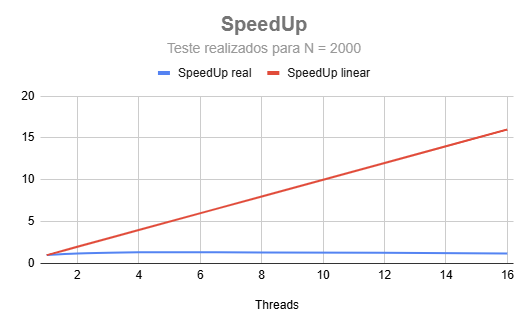
\includegraphics[width=0.70\textwidth]{imagens/speedup1.png}
    \caption{Gráfico de Speeedup}
    \label{fig:openmp-speedup}
\end{figure}

\begin{figure}[ht]  
    \centering
    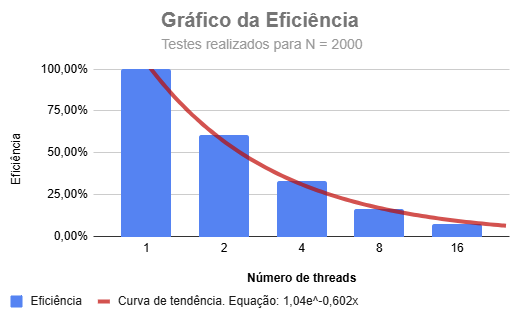
\includegraphics[width=0.70\textwidth]{imagens/eficiencia1.png}
    \caption{Gráfico de eficiência}
    \label{fig:openmp-eficiencia} 
\end{figure}

Contudo, pode-se observar que os resultados não foram satisfatórios, já que o \emph{speedup} não foi nem próximo do linear, e a eficiência foi caindo há medido do aumento do número de \emph{threads}. Isso pode ser explicado pela natureza do problema, que possui um alto grau de paralelismo. Ainda assim, a implementação paralela obteve um desempenho superior ao sequencial, com um \emph{speedup} máximo de 1.33 e eficiência de 33.25\%.


\subsection{CUDA}
Após as implementações realizadas e mostradas na seção \ref{sec:desenvolvimento}, foram realizados testes de desempenho para avaliar a eficácia da paralelização do modelo criado. As Figuras~\ref{fig:grafico_resultados-stencil2D} e \ref{fig:grafico_resultados-stencil1D} mostram os resultados obtidos para o \emph{Stencil} 2D e 1D, respectivamente.

\begin{figure}[ht]
    \centering
    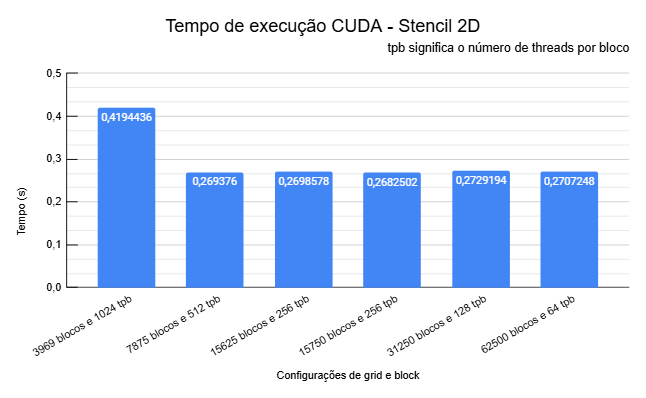
\includegraphics[width=0.75\textwidth]{imagens/grafico_resultados-stencil2D.png}
    \caption{Gráfico de desempenho do \emph{Stencil} 2D.}
    \label{fig:grafico_resultados-stencil2D}
\end{figure}

\begin{figure}[ht]  
    \centering
    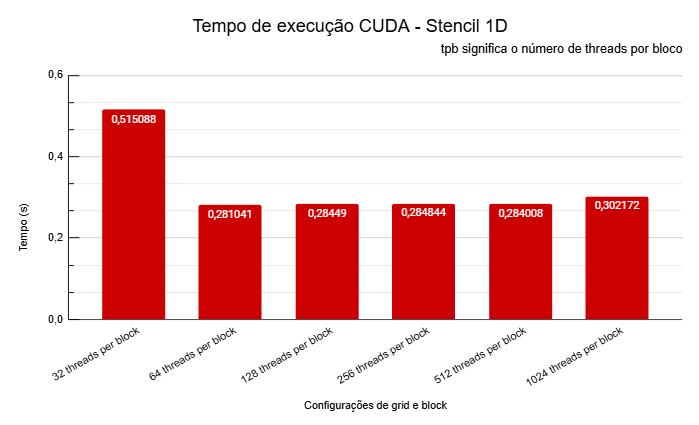
\includegraphics[width=0.75\textwidth]{imagens/grafico_resultados-stencil1D.png}
    \caption{Gráfico de desempenho do \emph{Stencil} 1D.}
    \label{fig:grafico_resultados-stencil1D}
\end{figure}

Diante os resultados da Figura \ref{fig:grafico_resultados-stencil2D} e \ref{fig:grafico_resultados-stencil1D}, pode-se verificar que os resultados para diversas configurações de \emph{grids} e \emph{blocks} foram satisfatórios, já que para um problema com um número expressivo de iterações, o tempo de processamento total está na ordem de milissegundos. Contudo, é possível observar que o \emph{Stencil} 2D obteve um desempenho superior ao \emph{Stencil} 1D, o que pode ser justificado pela complexidade do cálculo, que envolve mais operações matriciais. Ainda sobre os resultados do \emph{stencil} 2D, também pode-se observar que a configuração em que o número de blocos e o número de \emph{threads} por bloco são de 7875 e 512, respectivamente.

Já sobre o \emph{stencil} 1D, o desempenho também foi satisfatório mas inferior ao \emph{stencil} 2D, o que pode ser explicado pela forma como os dados são acessados na memória. A configuração que apresentou melhor desempenho foi com 16384 blocos e 256 \emph{threads} por bloco (64 \emph{threads} por bloco), resultando em um tempo de execução médio de 281 milissegundos.

Comparando as duas implementações, pode-se observar que ambas as abordagens atingiram resultados expressivos em termos de desempenho. O \emph{stencil} 2D demonstrou ser mais eficiente para este problema específico, possivelmente devido à melhor utilização da localidade espacial da memória e ao padrão de acesso aos dados mais otimizado. Por outro lado, o \emph{stencil} 1D, embora com tempos de execução ligeiramente superiores, ainda manteve um excelente desempenho, demonstrando que ambas as estratégias são viáveis para a resolução do problema.

A Tabela \ref{tab:comparacao_implementacoes} apresenta uma comparação entre as melhores médias das amostras quando implementadas em código sequencial, OpenMP e CUDA. Deve-se levar em consideração a confiabilidade dos resultados, já que o número de testes realizados foi superior a 30. Diante os resultados obtidos, a implementação que melhor performou foi a codificação utilizando a tecnologia CUDA, com um \emph{speedup} de 80.1603 em relação à implementação sequencial. Por fim, a eficiência da implementação em CUDA não foi calculada, já que a modelagem CUDA apresenta características únicas, quando comparadas às demais. Portanto, o cálculo da eficiência para tal arquitetura deve ser diferente e não foi considerado para esse trabalho. 

\begin{table}[ht]
    \centering
    \caption{Comparação entre as diferentes implementações}
    \begin{tabular}{|c|c|c|c|}
        \hline
        \textbf{Implementação} & \textbf{Tempo (s)} & \textbf{Speedup} & \textbf{Eficiência} \\
        \hline
        Sequencial & 21.507 & 1.00 & 1.00 \\
        \hline
        OpenMP & 16.1707 & 1.3300 & 0.3325 \\
        \hline
        CUDA 1D & 0.2810 & 76.5374 & - \\
        \hline
        CUDA 2D & 0.2683 & 80.1603 & - \\
        \hline
    \end{tabular}
    \label{tab:comparacao_implementacoes}
\end{table}

Por fim, assim como realizada nos resultados para o \emph{OpenMP}, a Figura \ref{fig:speedupCUDA1D} mostra o \emph{speedup} obtido para a implementação com o \emph{stencil} 1D, e a Figura \ref{fig:speedupCUDA2D} mostra o \emph{speedup} obtido para a implementação com o \emph{stencil} 2D. As ilustrações podem ser utilizadas para comparar os \emph{speedups} encontrados em cada um dos paradigmas implementados de paralelismo. Para qualquer comparação, deve-se saber que o tempo de referência utilizado para calcular os \emph{speedups} foi o tempo de execução da implementação sequencial, de 21.507 segundos.

\begin{figure}[ht]
    \centering
    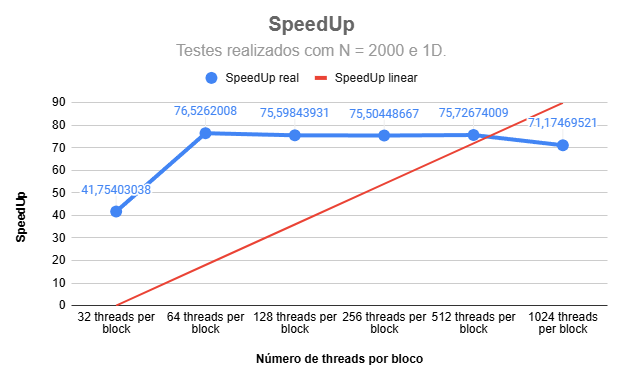
\includegraphics[width=0.75\textwidth]{imagens/speedupCUDA-1D.png}
    \caption{Gráfico de \emph{speedup} para o \emph{stencil} 1D.}
    \label{fig:speedupCUDA1D}
\end{figure}

\begin{figure}[ht]  
    \centering
    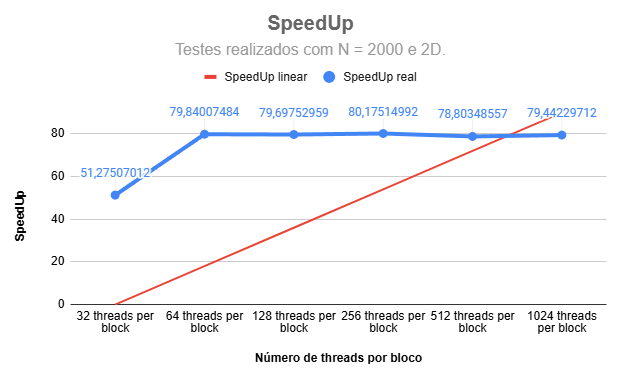
\includegraphics[width=0.75\textwidth]{imagens/speedupCUDA-2D.png}
    \caption{Gráfico de \emph{speedup} para o \emph{stencil} 2D.}
    \label{fig:speedupCUDA2D}
\end{figure}


\subsection{MPI}
Os resultados obtidos no experimento demonstram diferenças pouco significativas entre as implementações 1D e 2D no que se refere ao desempenho da paralelização. A decomposição 1D apresentou uma execução mais eficiente, com menor sobrecarga de comunicação, enquanto a 2D obteve uma redução de tempo mais expressiva, mas enfrentou desafios relacionados à escalabilidade devido à troca de dados entre múltiplos processos.

Ao analisar o speedup, a implementação 1D atingiu um valor próximo ao ideal com quatro processos, o que indica uma boa escalabilidade até esse número de processos. Já a decomposição 2D obteve um \emph{speedup} real máximo de aproximadamente 4,57 vezes com 4 processos. Isso pode ser explicado pelo aumento no número de vizinhos na memória, já que a abordagem 2D possui vizinhos em quatro direções.

\begin{figure}[ht]
    \centering
    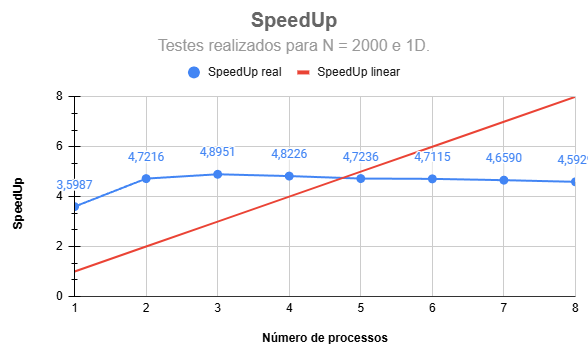
\includegraphics[width=0.75\textwidth]{imagens/speedupMPI-1D.png}
    \caption{Gráfico de \emph{speedup} para o \emph{stencil} 1D.}
    \label{fig:speedupMPI1D}
\end{figure}

\begin{figure}[ht]  
    \centering
    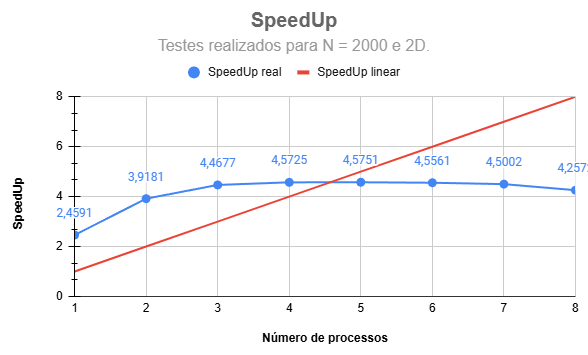
\includegraphics[width=0.75\textwidth]{imagens/speedupMPI-2D.png}
    \caption{Gráfico de \emph{speedup} para o \emph{stencil} 2D.}
    \label{fig:speedupMPI2D}
\end{figure}

Já sobre os tempos, as Figuras \ref{fig:tempoMPI1D} e \ref{fig:tempoMPI2D} mostram os tempos de execução para as implementações do \emph{stencil} 1D e 2D, respectivamente. Com base nos resultados, pode-se observar que os tempos para 1D e 2D ficaram bem próximos, com uma pequena vantagem para o \emph{stencil} 1D. Contudo, a diferença entre os tempos de execução não foi significativa, o que sugere que ambas as implementações são eficientes e apresentam um bom desempenho.

\begin{figure}[ht]
    \centering
    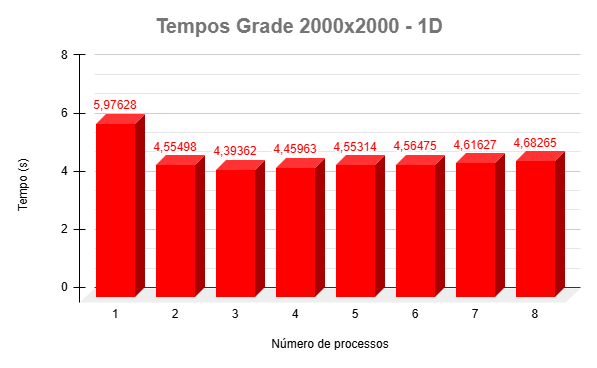
\includegraphics[width=0.75\textwidth]{imagens/tempoMPI-1D.png}
    \caption{Gráfico do tempo para o \emph{stencil} 1D.}
    \label{fig:tempoMPI1D}
\end{figure}

\begin{figure}[ht]  
    \centering
    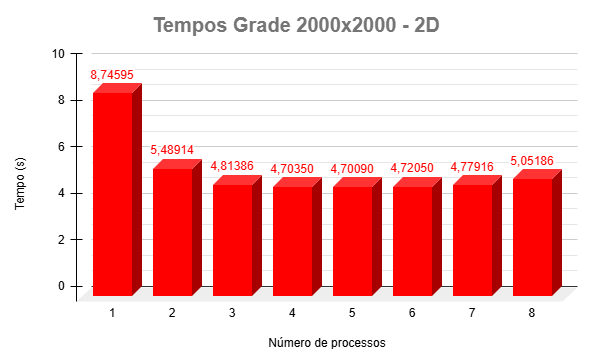
\includegraphics[width=0.75\textwidth]{imagens/tempoMPI-2D.png}
    \caption{Gráfico do tempo para o \emph{stencil} 2D.}
    \label{fig:tempoMPI2D}
\end{figure}

Conclui-se, portanto, que a decomposição 1D foi a abordagem sutilmente mais eficiente para o problema analisado, permitindo um ganho próximo ao ideal com o mínimo de sobrecarga, para o número de processos menor ou igual a 4. A decomposição 2D, embora tenha apresentado uma redução de tempo mais significativa, teve sua escalabilidade limitada pela necessidade de sincronização entre os processos. A escolha entre as abordagens deve levar em conta a relação entre simplicidade e potencial de paralelismo, com otimizações na comunicação podendo melhorar a performance da decomposição 2D em cenários mais amplos. Contudo, deve-se considerar que os valores de tempo basais utilizados para calcular o \emph{speedup} foi o tempo de execução da implementação sequencial, que foi de 21.507 segundos. Pensou-se nessa abordagem para que houvesse uma justiça nas comparações.

\subsection{Comparação entre as Implementações}
Devido as diferentes abordagens de paralelização, a comparação de \emph{benchmark} das metodologias é de difícil análise. Contudo, a Tabela \ref{tab:comparacao_implementacoes} apresenta uma comparação entre as melhores médias das amostras quando implementadas em código sequencial, OpenMP, CUDA e MPI. 

\begin{table}[ht]
    \centering
    \caption{Comparação entre as diferentes implementações}
    \begin{tabular}{|c|c|c|c|}
        \hline
        \textbf{Implementação} & \textbf{Tempo (s)} & \textbf{Speedup} & \textbf{Eficiência} \\
        \hline
        Sequencial & 21.507 & 1.00 & 1.00 \\
        \hline
        OpenMP & 16.1707 & 1.3300 & 0.3325 \\
        \hline
        CUDA 1D & 0.2810 & 76.5374 & - \\
        \hline
        CUDA 2D & 0.2683 & 80.1603 & - \\
        \hline
        MPI 1D & 4.3936 & 4.8951 & 1.6316 \\
        \hline
        MPI 2D & 4.7009 & 4.5751 & 0.9150 \\
        \hline
    \end{tabular}
    \label{tab:comparacao_implementacoes_finais}
\end{table}


% Seção da conclusão
\section{Conclusão} \label{sec:conclusao}
Devido aos resultados sumarizados na Tabela \ref{tab:comparacao_implementacoes_finais}, pode-se concluir que a implementação em CUDA 2D foi a mais eficiente, com um \emph{speedup} de 80.1603 em relação à implementação sequencial. A implementação em OpenMP obteve resultados pouco satisfatórios, obtendo, no melhor caso, uma eficiencia inferir à metade da referência utilizada. Já as implementações em MPI, embora tenham apresentado um desempenho satisfatório, não foram tão eficientes quanto as implementações em CUDA. A implementação 1D obteve um \emph{speedup} de 4.8951, enquanto a implementação 2D obteve um \emph{speedup} de 4.5751. Contudo, deve-se levar em consideração que a máquina utilizada para realizar os testes não tinha uma GPU capaz de realizar os cálculos em CUDA, o que pode ter influenciado nos resultados obtidos, pois usamos a \emph{engine} T3 do \emph{Google Colab}.

No mais, a implementação em CUDA foi a mais eficiente para o problema proposto, possuindo resultados expressivos até com o aumento no número de iterações e um aumento no número de iterações também. Já a abordagem em MPI, os resultados obtidos foram ótimos, pois foram executados em um \emph{laptop} de uso pessoal e obteve um \emph{speedup} de quase cinco vezes em relação à implementação sequencial.
% Seção das referências
\section{Referências} \label{sec:referencias}
\bibliographystyle{sbc}
\bibliography{sbc-template}


\end{document}